\documentclass[tikz,border=10pt]{standalone}
\usepackage{tikz}
\usetikzlibrary{shapes,arrows,positioning,calc,patterns,shadows,arrows.meta}

\definecolor{bertblue}{RGB}{66,133,244}
\definecolor{gptgreen}{RGB}{52,168,83}
\definecolor{vitpurple}{RGB}{142,36,245}
\definecolor{clporange}{RGB}{251,188,5}

\begin{document}
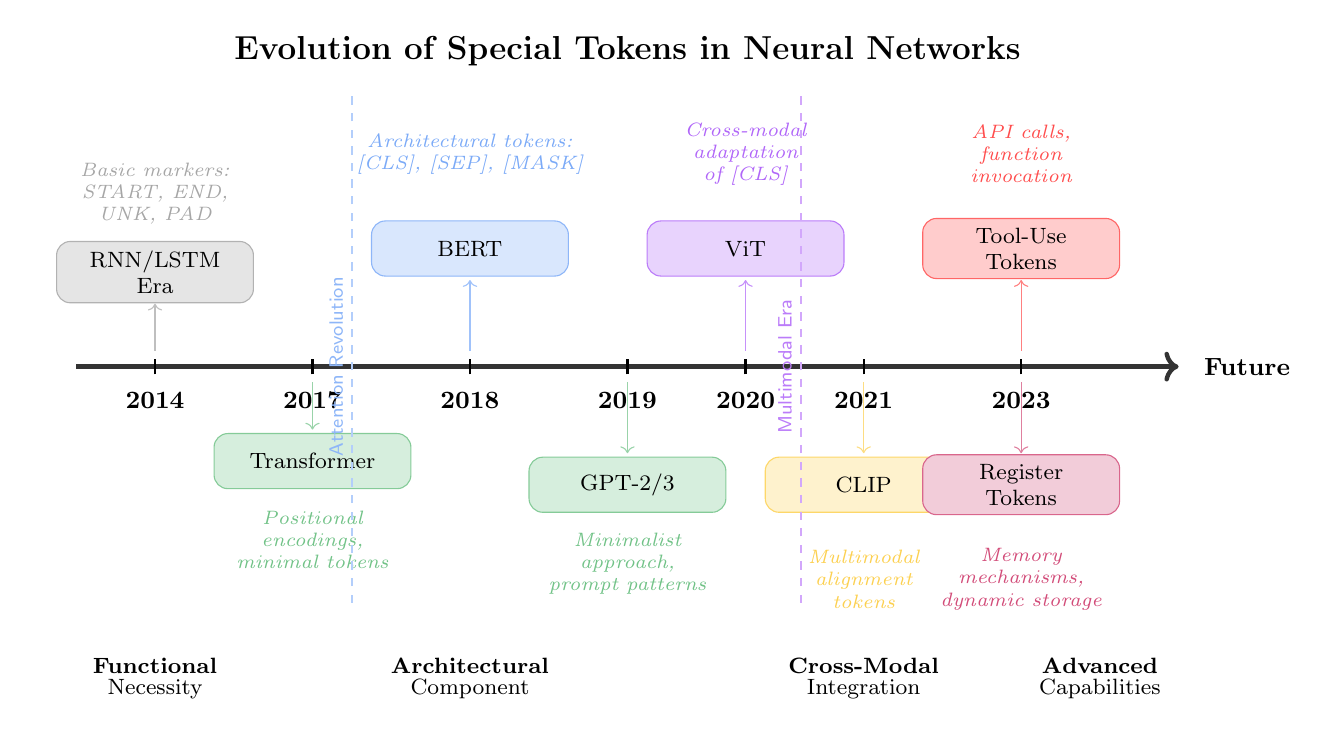
\begin{tikzpicture}[
    timeline/.style={ultra thick, black!80, ->},
    year/.style={font=\small\bfseries},
    event/.style={rectangle, rounded corners=5pt, minimum width=2.5cm, minimum height=0.7cm, font=\footnotesize, align=center},
    innovation/.style={font=\scriptsize\itshape, text width=3cm, align=center}
]

% Timeline arrow
\draw[timeline] (0,0) -- (14,0);
\node[year, anchor=west] at (14.2,0) {Future};

% Years
\foreach \year/\x in {2014/1, 2017/3, 2018/5, 2019/7, 2020/8.5, 2021/10, 2023/12} {
    \draw[thick] (\x, -0.1) -- (\x, 0.1);
    \node[year, anchor=north] at (\x, -0.2) {\year};
}

% Pre-transformer era
\node[event, fill=gray!20, draw=gray!60] at (1, 1.2) {RNN/LSTM\\Era};
\node[innovation, gray!70] at (1, 2.2) {Basic markers:\\START, END,\\UNK, PAD};
\draw[->, gray!50] (1, 0.2) -- (1, 0.8);

% Transformer
\node[event, fill=gptgreen!20, draw=gptgreen!60] at (3, -1.2) {Transformer};
\node[innovation, gptgreen!70] at (3, -2.2) {Positional\\encodings,\\minimal tokens};
\draw[->, gptgreen!50] (3, -0.2) -- (3, -0.8);

% BERT
\node[event, fill=bertblue!20, draw=bertblue!60] at (5, 1.5) {BERT};
\node[innovation, bertblue!70] at (5, 2.7) {Architectural tokens:\\{[CLS], [SEP], [MASK]}};
\draw[->, bertblue!50] (5, 0.2) -- (5, 1.1);

% GPT-2
\node[event, fill=gptgreen!20, draw=gptgreen!60] at (7, -1.5) {GPT-2/3};
\node[innovation, gptgreen!70] at (7, -2.5) {Minimalist\\approach,\\prompt patterns};
\draw[->, gptgreen!50] (7, -0.2) -- (7, -1.1);

% Vision Transformer
\node[event, fill=vitpurple!20, draw=vitpurple!60] at (8.5, 1.5) {ViT};
\node[innovation, vitpurple!70] at (8.5, 2.7) {Cross-modal\\adaptation\\of [CLS]};
\draw[->, vitpurple!50] (8.5, 0.2) -- (8.5, 1.1);

% CLIP
\node[event, fill=clporange!20, draw=clporange!60] at (10, -1.5) {CLIP};
\node[innovation, clporange!70] at (10, -2.7) {Multimodal\\alignment\\tokens};
\draw[->, clporange!50] (10, -0.2) -- (10, -1.1);

% Recent innovations
\node[event, fill=red!20, draw=red!60] at (12, 1.5) {Tool-Use\\Tokens};
\node[innovation, red!70] at (12, 2.7) {API calls,\\function\\invocation};
\draw[->, red!50] (12, 0.2) -- (12, 1.1);

% Register tokens
\node[event, fill=purple!20, draw=purple!60] at (12, -1.5) {Register\\Tokens};
\node[innovation, purple!70] at (12, -2.7) {Memory\\mechanisms,\\dynamic storage};
\draw[->, purple!50] (12, -0.2) -- (12, -1.1);

% Key transitions
\draw[dashed, thick, bertblue!40] (3.5, -3) -- (3.5, 3.5);
\node[rotate=90, font=\scriptsize\sffamily, bertblue!60] at (3.3, 0) {Attention Revolution};

\draw[dashed, thick, vitpurple!40] (9.2, -3) -- (9.2, 3.5);
\node[rotate=90, font=\scriptsize\sffamily, vitpurple!60] at (9.0, 0) {Multimodal Era};

% Title
\node[font=\large\bfseries] at (7, 4) {Evolution of Special Tokens in Neural Networks};

% Legend categories
\node[font=\footnotesize\bfseries] at (1, -3.8) {Functional};
\node[font=\footnotesize] at (1, -4.1) {Necessity};

\node[font=\footnotesize\bfseries] at (5, -3.8) {Architectural};
\node[font=\footnotesize] at (5, -4.1) {Component};

\node[font=\footnotesize\bfseries] at (10, -3.8) {Cross-Modal};
\node[font=\footnotesize] at (10, -4.1) {Integration};

\node[font=\footnotesize\bfseries] at (13, -3.8) {Advanced};
\node[font=\footnotesize] at (13, -4.1) {Capabilities};

\end{tikzpicture}
\end{document}